\begin{figure*}[t]
  \centering
  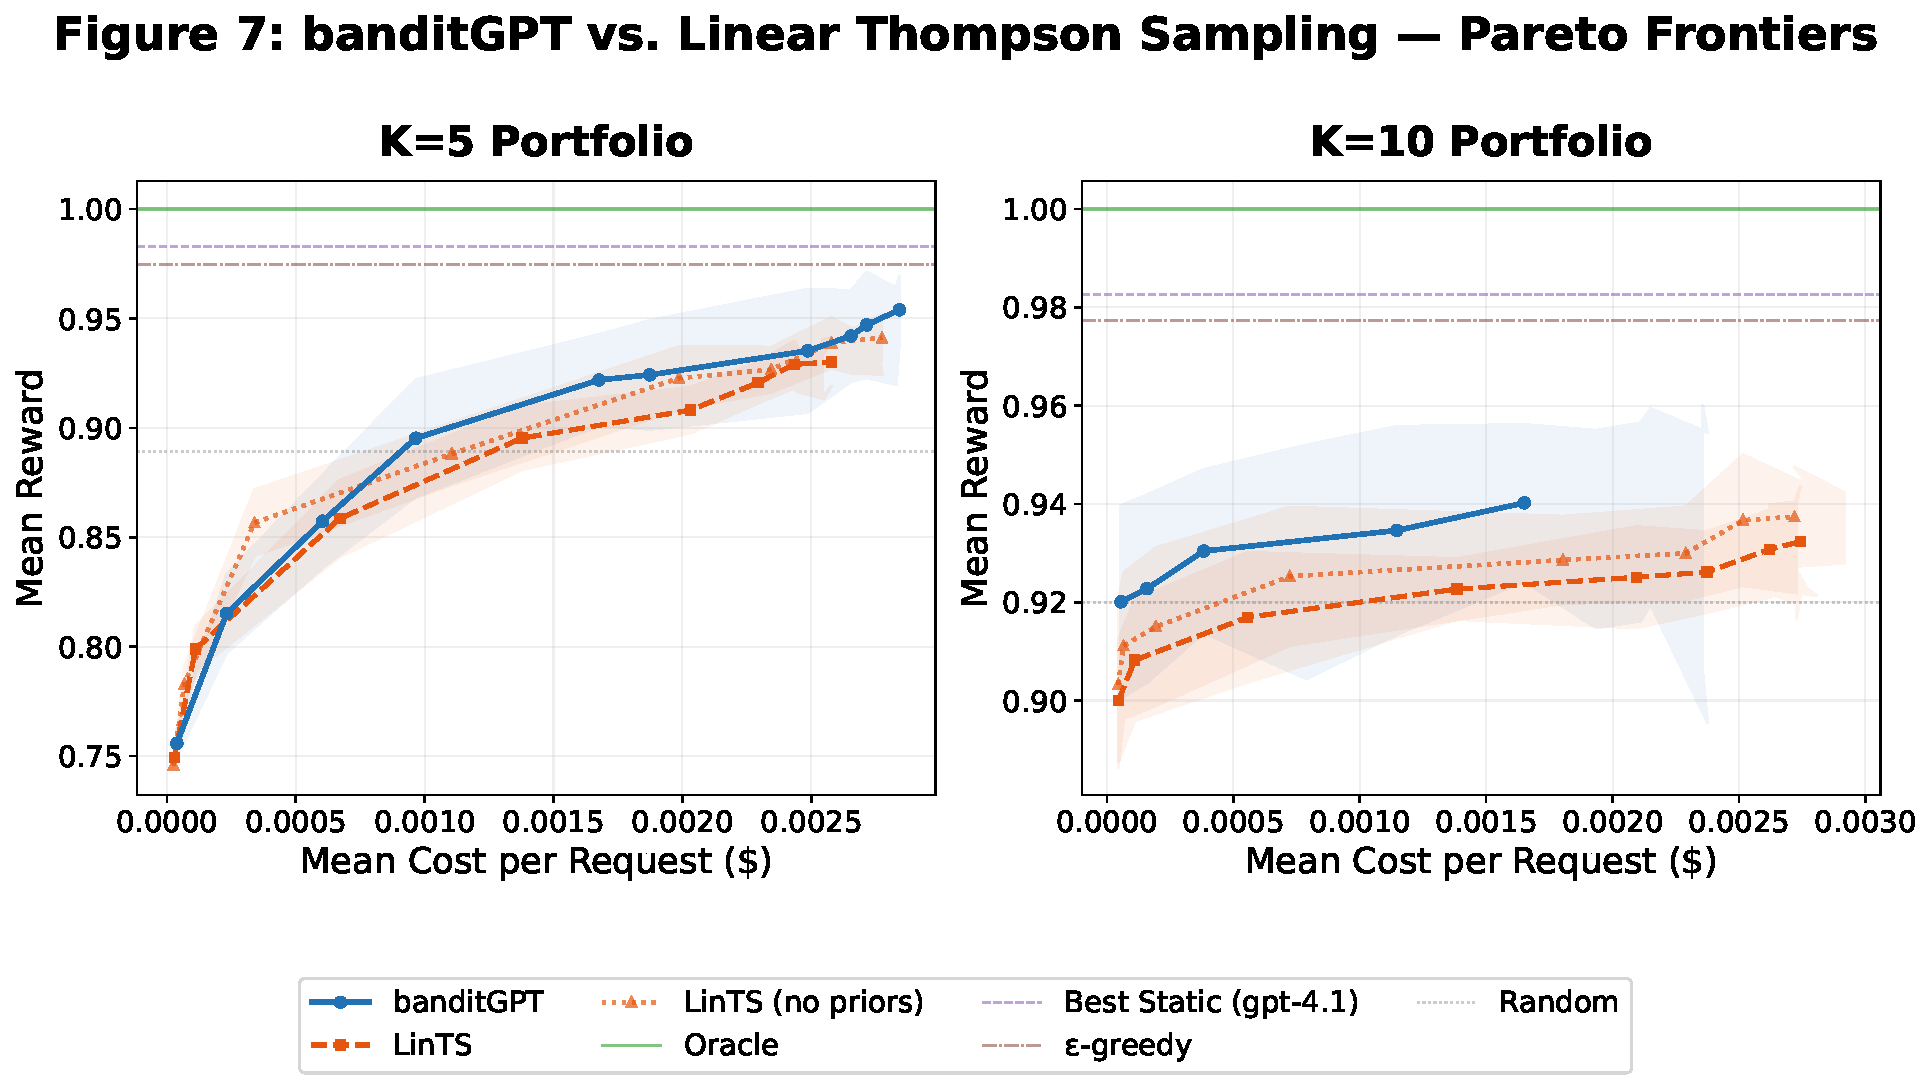
\includegraphics[width=\textwidth]{../experiments/07_figure/results/figure7_lints_comparison.pdf}
  \caption{
    \textbf{banditGPT vs.\ Linear Thompson Sampling (LinTS): Pareto Frontiers at $K{=}5$ and $K{=}10$.}
    Curves show quality--cost frontiers across $\lambda \in [0, 5]$ ($n{=}20$ trials, shaded bands: $\pm 1\sigma$).
    banditGPT (LinUCB + Corralling, solid blue) Pareto-dominates LinTS both with warmup priors (dashed orange) and without priors (dotted orange) across the cost spectrum.
    At $K{=}5$, the peak reward gap is 2.4~pp ($0.954$ vs.\ $0.930$, $p{<}0.05$); at $K{=}10$ it narrows to 0.8~pp ($0.940$ vs.\ $0.932$).
    Horizontal references show the per-prompt oracle, best single model (GPT-4.1, $0.983$), $\varepsilon$-greedy ($0.975$), and random routing.
    While the best static model leads at $\lambda{=}0$ (due to a small 1.7\% contextual ceiling), contextual routing finds cost-efficient allocations at nonzero $\lambda$ (Section~\ref{sec:egreedy_analysis}).
  }
  \label{fig:lints_pareto}
\end{figure*}
